%fichier : Projet_Di4_PPGL_Chana_Pecault.tex
%Date : 21/09/2021
%Version : 1.00
%Modif : 21/09/2021

\documentclass{EPUProjetDi}
\usepackage[bottom]{footmisc}

\makeindex

%remplir les lignes suivantes avec les informations vous concernant :
\title[Simulation d'une colonie de fourmis]{Simulation d'une colonie de fourmis}

\projet{Projet de Programmation et Génie Logiciel}

\author{
Narvin Chana\\ %Attention : toujours écrire d'abord le prénom puis le nom (ne pas mettre tout le nom en majuscules)
\noindent[\url{narvin.chana@etu.univ-tours.fr}]\\
Noé Pécault\\ %Attention : toujours écrire d'abord le prénom puis le nom (ne pas mettre tout le nom en majuscules)
\noindent[\url{noe.pecault@etu.univ-tours.fr}]}

\encadrant{Nicolas Monmarché\\ %
\noindent[\url{nicolas.monmarche@univ-tours.fr}]\\~\\
Polytech Tours\\
Département Informatique\\~ %
}

%%%%%%%%%%%%%%%%%%%%%%%%%%%%%%%%%%%%%%%%%%%%%%%%%%%%%%%%%%%%%%%%%%%%%%%%%%%%%%%%%%%%%%%%%%
\begin{document}

\maketitle

\pagenumbering{roman}
\setcounter{page}{0}

{
%on réduit momentanément l'écart entre paragraphes pour ne pas trop aérer la table des matières
\setlength{\parskip}{0em}

\tableofcontents

%\listoffigures
%rq1 : si vous n'avez pratiquement pas de figures, laissez la ligne précédente en commentaire

%\listoftables
%rq1 : si vous n'avez pratiquement pas de tables, laissez la ligne précédente en commentaire
}


\start
%%%%%%%%%%%%%%%%%%%%%%%%%%%%%%%%%%%%%%%%%%%%%%%%%%%%%%%%%%%%%%%%%%%%%%%%%%%%%%%%%%%%%%%%%%

\chapter*{Introduction}
%le 2 lignes suivantes permettent d'ajouter l'introduction à la table des matières
%et d'afficher "Introduction en haut des pages"
\addcontentsline{toc}{chapter}{\numberline{}Introduction}
\markboth{\hspace{0.5cm}Introduction}{}

\paragraph{}
Le problème de la simulation et de l'optimisation d'une colonie de fourmis est un problème complexe 
qui met en oeuvre des connaissances dans les domaines de la théorie des graphes, la recherche opérationnelle 
et dans les systèmes décentralisés. Chaque fourmi agi par elle même et l'ensemble des fourmis forme une intelligence
à part entière qui n'a pas de cerveau centralisé.

Ses applications sont vastes et interviennent dans des domaines tels que les problèmes d'ordonnancements, 
de routage (ex: réseau Internet ou tournée de véhicules) ou encore le traitement d'image (ex: détection de bords).

Ce problème de simulation de colonie de fourmis nous intéresse depuis longtemps et c'est donc pour cela que dans 
le cadre du projet de programmation et génie logiciel nous avons choisi de proposer un sujet qui traite de celui-ci.

Notre objectif pour ce projet était de créer une application permettant de simuler les interactions qu'une colonie 
de fourmis peut avoir avec son environnement. Les fourmis doivent pouvoir explorer les alentours de leur colonie afin 
de trouver de la nourriture et de la ramener à sa colonie. 
Nous avions aussi imaginé d'autres fonctionnalités qui pourraient venir se greffer au projet si le temps nous le permettait
comme des combats entre fourmilières et la possibilité de simuler plusieurs colonies.

En revanche, il n'était pas dans nos objectifs de simuler l'intérieur de la colonie et n'est pas voué à être sur le long terme
(nous ne prenions donc pas en compte la durée de vie des fourmis).

Il nous était également très important de respecter les principes de génie logiciel qui nous ont été appris durant notre
parcours à Polytech dans le but de développer une application robuste et facilement extensible.

Au sein de ce rapport, nous présenterons notre démarche pour arriver aux objectifs fixés, le déroulement du projet ainsi que les résultats 
et ce dont on en a tiré.

\chapter{Conception et décisions}

Ce chapitre traite des objectifs et contraintes du projet, de son architecture et des interactions entre les différents modules. 
Nous y détaillons aussi les différentes entités et structures qui appartiennent à la simulation ainsi que la structure de la partie applicative.

\section{Objectifs et contraintes}

\subsection*{Système décentralisé}

Un système décentralisé \footnote[1]{Page wikipedia \url{https://en.wikipedia.org/wiki/Decentralised_system}} est un système composé de sous-composants qui accomplissent des objectifs individuellement afin
de réussir un objectif global.
Les entités qui composent le système doivent interagir entre elles non pas via une intelligence globale mais par des moyens
de communication plus locaux.

Le problème de la simulation de colonie est une application typique de ce principe et se retrouve même dans la nature.
Dans une vraie fourmilière, il n'y a aucune entité qui donne les ordres aux autres et donc chaque fourmi connaît sa mission
pour faire prospérer la colonie. 

Il est donc essentiel pour notre simulation de respecter cette architecture et chaque fourmi doit donc prendre ses décisions
avec seulement les informations qui lui sont accessibles.

\subsection*{Simulation personnalisable}

La simulation doit aussi être un outil facile à utiliser afin de tester des configurations initiales différentes.
Il en va de même pour les constantes de simulation comme la portée de perception des fourmis, leur vitesse et toutes les autres.

Nous cherchons donc à avoir une interface graphique simple à utiliser qui permettra de placer les éléments de la simulation à la guise
de l'utilisateur.

\subsection*{Séparation Moteur et Application}

Une des contraintes clés du projet est la séparation de la partie \textbf{Moteur de simulation} et \textbf{Application}.
Cela permet de réutiliser ce moteur pour d'autres applications comme par exemple pour générer des trajectoires des fourmis 
pour une animation.

Cela nous contraint donc à faire en sorte que le moteur n'ait absolument aucune dépendance envers la partie application.

\subsection*{Abstraction des entités pour l'évolutivité}

Nous avons intérêt à garantir une certaine évolutivité de la simulation car le comportement des fourmis que nous avons conceptualisé
n'est pas forcément exact et nous devions nous permettre de facilement le changer.

Il est même aussi possible que nous souhaitions utiliser ce même moteur pour simuler des comportements autre que
des fourmis ce qui force un certain niveau d'abstraction.

\subsection*{Optimisation future}

La simulation de colonie de fourmis est un problème très gourmand en termes de ressources de calcul car il est nécessaire de calculer les mouvements
de chaque fourmi à une cadence assez élevé pour atteindre un taux de mise à jour par seconde proche suffisant pour que la simulation paraisse fluide 
(60 images par secondes).

Une piste d'optimisation dont nous avons eu conscience au moment de la conception est de paralléliser le calcul des fourmis tout en s'assurant de maintenir
l'intégrité des résultats de la simulation (pas de problème de concurrence).

Nous cherchons donc une architecture nous ouvrant la possibilité d'implémenter facilement une telle technique d'optimisation sans avoir à
refaire l'architecture de 0. 

\pagebreak

\section{Moteur}

\subsection{Structure générale}

Le moteur de simulation est donc là où les calculs de trajectoire et de décisions des fourmis seront effectués.
Sa structure est simple et est très largement inspiré de ce qu'on peut trouver dans le domaine du jeu vidéo et 
cela n'est pas étonnant car notre simulation se rapporte beaucoup à un jeu vidéo.

Tout d'abord, les individus de notre simulation sont des \textbf{Entités}. Une entité est un objet associé à un
\textbf{Transform} qui représente un état physique dans le monde (position, rotation, taille) et aussi d'un comportement
qui lui est défini dans une méthode Update() sous la forme d'une suite d'instructions.

Cet objet Transform\footnote{Page du manuel d'Unity sur l'objet Transform \url{https://docs.unity3d.com/Manual/class-Transform.html}} 
est une inspiration directe du jeu vidéo et plus précisément du moteur de jeu Unity

On a l'objet qui sert de chef d'orchestre à la simulation qui est le \textbf{Monde}. Il possède les propriétés concernant 
l'environnement des fourmis et contient aussi la totalité des entités présentent dans la simulation.
Lorsqu'il est mis à jour, le monde doit donc mettre à jour la totalité des entités qu'il contient pour que chaque entité 
puisse exécuter ses actions.

\begin{figure}[h]
    \centering
    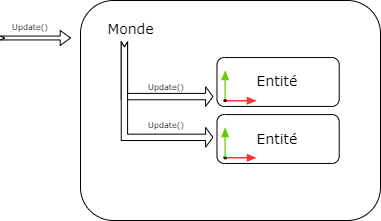
\includegraphics[scale=0.8]{moteur_structuregenerale.png}
    \caption{Flux de mise à jour}
    \label{fig:flow_update}
\end{figure}

\autoref{fig:flow_update} montre le processus de mise à jour de la simulation qui commence  par le monde et 
qui est distribuée à toutes les entités qu'il contient.

\pagebreak
\subsection{Entités}

\subsubsection*{Définition}

Ce que nous appelons \textbf{Entité} est un objet possédant un état physique qui est composé d'une position, une rotation et une taille (\textbf{Transform}) 
ainsi que d'une logique interne que l'on appellera comportement.

Cette association de position, rotation et d'une taille est ce qu'on appelle un \textbf{Transform} et caractérise l'existence dans le monde de l'entité.
La définition de cet objet nous est utile car elle nous permet de manipuler l'état de l'entité dans une même structure et d'appliquer des transformations
linéaires simplement dans le cas où l'on voudrait faire un système de coordonnées relatif à une autre entité.

Les entités sont les briques essentielles à la simulation car elles représentent les objets de notre simulation. 

\subsubsection*{Spécialisations des entités}

La classe \textbf{Entity} est donc la version la plus abstraite d'un de ces objets et chacune de ses spécialisations
représentera une entité au comportement différent pouvant exister dans la simulation.

Les comportements ajoutés sont par exemple le système de vie, une machine à états ou même le comportement d'une fourmi.
Le dernier composant présent dans chaque entité est le \textbf{Collider} qui est la boîte de collision d'une entité et peut se définir 
de différentes formes selon les besoins. Il est utile dans le calcul des mouvements car il permet de tester si une entité ne cherche pas 
à se déplacer dans un mur.

\autoref{fig:struct_entities_spec} montre l'arborescence des entités avec ce que chacune apporte comme fonctionnalité.

\begin{figure}[h]
    \centering
    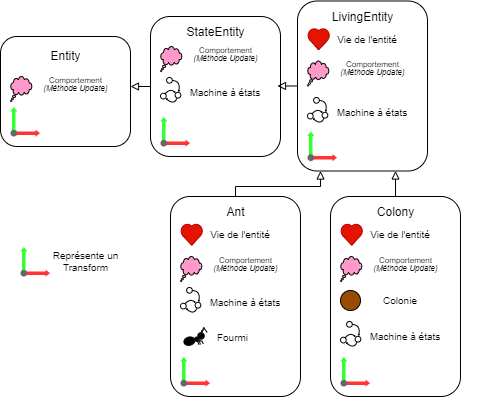
\includegraphics[scale=0.5]{entities_specialisations.png}
    \caption{Diagramme des spécialisations des entités avec leurs apports}
    \label{fig:struct_entities_spec}
\end{figure}

\subsection{World}

\subsubsection*{Définition}

Le monde est l'espace dans lequel la simulation se déroule et possède donc les propriétés de taille de la simulation ainsi que le Collider
gérant les murs de la simulation.
C'est lui qui stocke toutes les entités présentent dans la simulation et s'occupe de les mettre à jour lorsqu'il est lui-même mis à jour. 
\ref{fig:flow_update}

Par souci d'optimisation, le monde est divisé en régions qui sont chacune une liste des entités présentes dans la région. 
Cela permet de ne pas avoir à chercher des éléments parmi la liste complète de toutes les entités du monde.
Le monde est donc responsable du maintient de la cohérence de ces régions et met à jour toutes ces listes en fonction des positions
des entités à chaque instant T.

\begin{figure}[h]
    \centering
    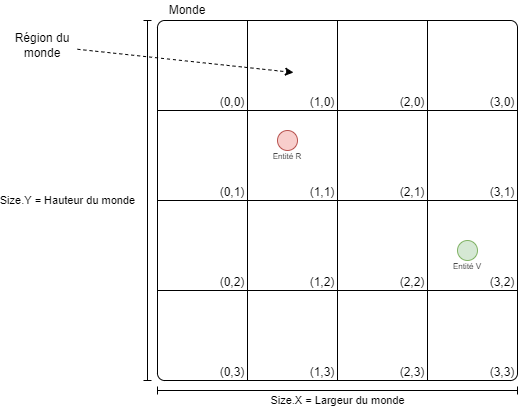
\includegraphics[scale=0.5]{world.png}
    \caption{Schéma d'un monde avec ses régions}
    \label{fig:world_scheme}
\end{figure}

Les murs de la simulation sont représentés par le WorldCollider qui est un second découpage (indépendant des régions) ayant pour but 
de stocker les cases traversables ou non par les autres entités.
Cette représentation des murs sous forme d'une matrice de booléens nous permet d'avoir une structure analogue à une image ayant pour chaque pixel
une valeur \textbf{Vrai} pour représenter un mur ou \textbf{Faux} pour représenter une case traversable.

\begin{figure}[h]
    \centering
    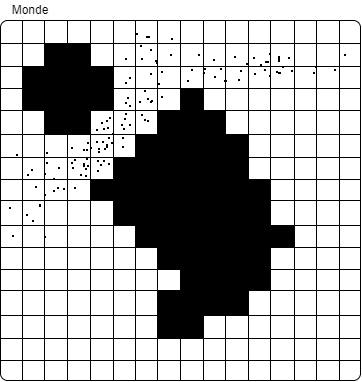
\includegraphics[scale=0.4]{world_colliderdrawio.png}
    \caption{Schéma d'un monde avec ses murs }
    \label{fig:world_collider_scheme}
\end{figure}


\subsection{Colliders}

\subsection{Fourmis}

\subsubsection{Comportement d'une fourmi}

\subsubsection{Machine à états}

\paragraph{}
Durant le projet, nous nous sommes inspirés des cours de génie logiciel afin d'utiliser des design patterns pour répondre à des problèmes.

\paragraph{}
Le premier réel problème de design que nous avons découvert était en relation avec la manière de mettre en code les différents états que la fourmi peut avoir.
La solution "évidente" à ce problème est le design pattern \textit{State} (États).
Cela nous a permis d'isoler les différents comportements que la fourmi peut avoir et donc de rendre plus facile la relecture de code et le debugging.
Sans utiliser ce design pattern, le code serait très rapidement devenu illisible et il aurait été beaucoup plus compliqué de rajouter des états.

\paragraph{}
L'autre problème que nous avons relevé après la phase de conception initiale est par rapport aux mouvements de la fourmi. 
Dans certains cas il peut être utile d'implémenter rapidement des stratégies différentes sans pour autant changer des gros morceaux de codes afin d'en faire une comparaison de leurs efficacité.
C'est ici que le design pattern \textit{Strategy} (Stratégie) intervient. Il permet de rapidement comparer des méthodes de déplacement en attribuant à chaque colonie (ou même à un ensemble de fourmis) une
stratégie de déplacement.
Malheureusement, nous n'avons pas eu le temps d'implémenter des stratégies autres que LineStrategy\footnote{Déplacement dans la direction moyenne de la PerceptionMap.} 
et WandererStrategy\footnote{Déplacement dans la direction dominante de la PerceptionMap influencée par une variable aléatoire.}.


\subsubsection{Colonie}

\subsubsection{Ressources}

\subsubsection{Pheromones}

\subsubsection{Entité vivante qui se déplace}


\section{Application}

\subsection{Présentation de la structure}

\subsubsection{Elements d'interface}

\chapter{Réalisation}

\paragraph{}
Ce chapitre présente le déroulement du projet, les aléas qui sont apparus au cours du 
développement et d'autres aspects de développement qu'il nous a semblé 
utile de faire apparaître.

\section{Choix des outils et technologies}

\subsection{Outils de collaboration}

\paragraph{}
Lors des projets de 3\textsuperscript{ème} année, nous avons beaucoup appris sur comment utiliser
Git. Nous avons choisi d'utiliser \textbf{GitHub} en tant qu'outil de versionnage en raison de notre aise avec et
car le site possède un grand nombre de fonctionnalités nous permettant de mieux communiquer entre
nous.

\paragraph{}
Lors du projet nous avons adopté une méthode de travail basé sur le \textbf{GitFlow}\footnote{Une méthode de travail où on sépare chaque feature ou fix dans une branche séparée.
Ensuite une fois la feature finie, on créé un \textit{Merge Request} afin de demander la validation des autres développeurs.} avec pour seule nuance que nous n'avions pas de branches \textit{dev} ou \textit{release}
mais plutôt toute modification se fusionnait directement à la branche \textit{main}.

Cela avait pour avantage de nous permettre de suivre les avancements de l'autre personne et de pouvoir 
apporter des suggestions ou des commentaires sur ce qui a été fait. 
En fin de compte l'utilisation de ce workflow nous a permis de connaître et comprendre 
les parties de codes que l'autre écrit et donc de pouvoir beaucoup avancer chacun de notre
côté en ne laissant pas l'autre personne à l'abandon.

\begin{figure}[h!]
\centering
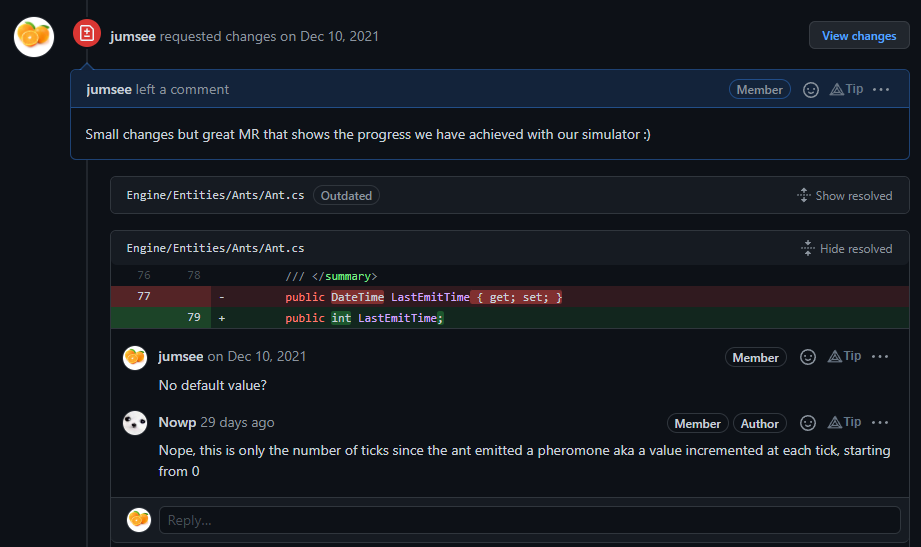
\includegraphics[scale=.5]{merge_request.png}
\caption{Exemple de commentaire sur un merge request pour l'ajout de la disparition des phéromones.}
\label{fig:MergeRequest}
\end{figure}

\paragraph{}
En plus des merge requests, GitHub nous permet de créer des \textit{issues}.
Ces \textit{issues} peuvent être considérés comme des tâches qu'il reste à faire. Au sein de GitHub, nous
pouvons à tout moment nous approprier une tâche afin d'indiquer qu'on a commencé à travailler dessus. Cela 
permet de bien savoir ce sur quoi l'autre personne travaille et également d'avoir un aperçu rapide de ce qu'il reste à faire dans le projet.

\paragraph{}
Il est évident que le nombre d'issues que nous avions au début du projet n'est pas le même qu'à la fin. Au cours du projet nous
pouvions découvrir des aspects du code à réparer (dans ce cas l'issue serait plutôt un \textit{bug report}) ou encore des fonctionnalités
importantes auxquelles nous n'avions pas pensés.

\paragraph{}
Les issues nous ont également permis de débattre entre-nous sur quelle serait la meilleure solution à un problème. Essentiellement, toute utilisation
de GitHub est dans l'objectif de faciliter la communication et le fait que tout soit bien répertorié nous assure de ne pas oublier des échanges que 
nous aurions pu avoir.

\paragraph{}
Ces issues apparaissent au sein de Kanbans \footnote{Au sein de ce projet le Kanban était notre tableau de bord et nous permettait de suivre 
l'avancement et de savoir ce qu'il restait à faire. Plus d'informations : \url{https://en.wikipedia.org/wiki/Kanban_(development)}.}
qu'on retrouve directement intégré à GitHub. Nous avions deux Kanbans, un pour l'Application et l'autre pour le moteur de simulation comme ces deux éléments peuvent avancer très facilement en parallèle.

\begin{figure}[h]
\centering
\includegraphics[scale=.4]{kanban.png}
\caption{Exemple du tableau de bord côté Application. 
\\On voit les tâches qui sont en cours de développement et ceux qui sont prêts à être review.}
\label{fig:Kanban}
\end{figure}

\paragraph{}
Un autre élément que nous avons utilisé avec GitHub est la fonctionnalité d'intégration continue. En effet, nous avons configuré notre projet 
pour lancer tous les tests unitaires à chaque commit effectué sur une branche.
Cela nous a permis de repérer des erreurs dans notre code car nous avons configuré le repo GitHub pour ne pas avoir le droit de merge une branche lorsque les tests unitaires ne passent pas.
En plus de cela, nous n'avions pas le droit de faire des commits directement sur la branche main et pour merge une branche il fallait la validation de l'autre personne.
Tout cela nous a apporté une connaissance plus générale sur le projet.

\subsection{Langages et Langues}

\paragraph{}
Le choix du langage de programmation à utiliser était une décision importante à prendre. Nous avons décidé de faire ce projet en C\# car c'est un langage que nous
n'avons pas encore pu utiliser au sein du parcours à Polytech. Nous étions au courant du fait que le C\# était très proche du Java et donc il n'y avait pas
d'inquiétudes sur notre capacité à l'apprendre rapidement. Le C\# reprend aussi les concepts de machine virtuelle qui existent en Java ce qui permettrait de build et lancer le projet
sur n'importe quel système d'exploitation grâce à .NET.
De plus, le C\# est un langage que nous avions pu utiliser lors de petit projets sur Unity mais jamais sur un gros projet comme celui-ci. 
A l'intérieur de C\# le standard de \hyphenation{docu-ment-ation} utilisé est XMLdoc\footnote{Plus d'informations : \url{https://docs.microsoft.com/en-us/dotnet/csharp/language-reference/xmldoc/}.}.

\paragraph{}
Ensuite, il a fallu que nous nous décidions sur quelle convention de nommage nous allions utiliser. 
Malgré notre envie d'utiliser celle présenté par notre enseignant en cours de C++ en 3\textsuperscript{ème} année, nous avons découvert la convention 
proposée par Microsoft pour le C\#\footnote{Plus d'informations : \url{https://docs.microsoft.com/en-us/dotnet/csharp/fundamentals/coding-style/coding-conventions}} qui nous a particulièrement plu.
Dans une volonté de vouloir rester polyvalent et malléable en terme de méthodes de travail, nous avons décidé d'adopter cette convention.

\paragraph{}
Pour ce qui est de la langue dans laquelle nous avons codé, nous avons décidé de tout faire en Anglais pour que le code soit facilement
transmissible et exploitable par d'autres individus dans le monde, chose qui dans le contexte de la mondialisation reste très important.

\subsection{Librairie de Tests}

\paragraph{}
Il existe plusieurs librairies de test au sein de l'environnement .NET. Les plus utilisés sont XUnit, NUnit et MSTest.
La bibliothèque que nous avons choisi d'utiliser est XUnit en raison du fait que Noé l'avait déjà utilisé au sein d'un projet personnel.

\subsection{Framework d'affichage}

\paragraph{}
Au lancement du projet, nous avons dû réfléchir à quel framework utiliser pour faire l'affichage de la simulation.
Dans un premier temps, nous nous étions intéressé à Avalonia, un framework cross-platform qui est un successeur spirituel de WPF\footnote{WPF ou Windows Presentation Foundation est un framework 
utilisé pour la création d'interfaces graphique. Aujourd'hui ce framework a beaucoup vieilli et est en train d'être remplacé par des frameworks plus modernes tels que Avalonia.}.
On s'est rendu compte qu'Avalonia n'était pas du tout ce qu'on recherchait comme il ne servait qu'à faire des interfaces graphiques et était très peu utilisable pour l'affichage de formes plus complexes.

\paragraph{}
Nous avons donc dû rechercher une solution alternative et c'est là que nous avons découvert MonoGame. 
MonoGame est un framework graphique open-source utilisé principalement pour des jeux comme son nom l'indique et qui est basé
sur XNA (un framework développé par Microsoft et abandonné depuis 2013). 
Après avoir consulté la documentation et avoir fait des recherches dessus, MonoGame est le framework que nous avons décidé d'utiliser. 
Il nous a permis de rendre plus simple certains aspects tels que l'importation et l'utilisation de textures.

\paragraph{}
En complément de MonoGame, l'ensemble des textures présents dans le projet ont été créé à la main avec Piskel\footnote{Outil gratuit de dessin de PixelArt en-ligne. 
Plus d'informations : \url{https://www.piskelapp.com/}.}. 

\section{Moteur}

\subsection{Abstraction des Colliders}

\paragraph{}
Lorsque nous avons codé les colliders, nous nous sommes rendu compte que la manière initiale dont nous l'avions conçu
faisait qu'il y avait énormément de duplication de code ce qui le rendait difficilement maintenable.

Exemple : Pour tester la collision entre un cercle et un rectangle il y a deux cas. Premier cas : le cercle appelle sa méthode CheckCollision en passant le rectangle en paramètre.
Second cas : 

La solution à cela était de déplacer les méthodes de collision dans une classe statique et qu'ensuite chaque collider fasse appel à la méthode qu'il a besoin dans la classe statique.

\subsection{Transforms et Colliders}
\paragraph{}
Comme indiqué précédemment, l'objet Transform que nous avons utilisé est inspiré de celui qu'on retrouve en Unity. Un autre concept que nous avons voulu reprendre de Unity est le fait qu'un
collider puisse posséder son propre transform ce qui lui permet d'avoir une position autre que celle de l'entité à la quelle il est attaché. Ca permet aussi aux colliders d'exister sans être forcément
lié à une entité.

\paragraph{}
Au début du projet, nous avions pour intention d'implémenter cela dans le moteur de simulation. 
Un collider aurait donc un transform et s'il est rattaché à une entité, le transform du collider serait en coordonnées relatives (pour obtenir sa position réelle, il faudrait faire Entity.Transform + Collider.Transform).
Il s'avère que cette solution ajoute beaucoup de complexité aux calculs de collision et ne serait même pas utile au sein de la simulation. Nous avons donc pris la décision d'enlever cette 
fonctionnalité et de lier fortement les colliders aux entités en lui faisant prendre le transform de l'entité auquel il est rattaché.

\subsection{Temps de simulation ou temps réel ?}
\paragraph{}
Une erreur gigantesque que nous avons commises est le fait que nous avons ajouté des éléments qui dépendaient du temps réel dans le moteur de simulation (un exemple serait le temps de disparition des phéromones).
Le problème ici vient du fait que nous voulions permettre aux utilisateurs de ralentir, accélérer ou mettre en pause la simulation.

\begin{figure}[h]
    \centering
    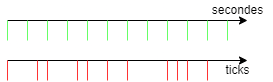
\includegraphics[scale=1]{ticks_secondes.png}
    \caption{Exemple d'appels de la méthode Update en temps réel et en temps de simulation.}
    \label{fig:ticks_secondes}
\end{figure}

Les lignes rouges dans \ref{fig:ticks_secondes} représentent des appels à Update. On voit que la méthode update n'est pas appelé de manière uniforme ce qui cause des décalages si on tente de changer la vitesse de la simulation.

Malheureusement, mettre en pause la simulation ne met pas en pause la vrai vie ! Il y a donc une désynchronisation qui se déroule et qui peut causer des problèmes de cohérence et d'intégrité.
La solution à ce problème est évidente, il faut décompter tout en nombre de \textit{ticks}, c'est à dire, de fois où la méthode Update du World est appelée. 
Cela fait que chaque phéromone possède un compteur pour sa disparition qui décroît de un à chaque Update. Cela permet de garder la cohérence dans le cas de modification de la vitesse de la simulation.

\subsection{Optimisation}

\paragraph{}
La problématique de l'optimisation de la simulation a été un enjeu très important pour nous tout au long du projet. Nous avons dû réfléchir sur les implémentations qui ont été faites afin de vérifier qu'elles ne 
faisaient pas chuter les performances. Que ce soit au niveau de quel type d'objet nous utilisions du C\# ou encore vérifier qu'on ne remplissait pas inutilement le garbage collector 
\footnote{Le garbage collector est un gestionnaire de mémoire qui supprime et désalloue automatiquement des objets quand ils ne sont plus référencés par le programme. 
Plus d'informations sur comment il fonctionne en .NET : \url{https://docs.microsoft.com/en-us/dotnet/standard/garbage-collection/fundamentals}}.
Quand on parle de simuler une quantité de fourmis qui peut aller dans les milliers, sachant que chaque fourmi doit évaluer son environnement et prendre des décisions, la performance chute très rapidement.

Nous présenterons dans cette partie les principales optimisations que nous avons effectués pour augmenter au maximum le nombre de fourmis que le simulateur peut supporter.

\subsubsection{Découpage par régions}
\paragraph{}
Le découpage par régions est l'optimisation la plus "simple" mais évidente que nous avons ajouté.

\begin{figure}[h]
    \centering
    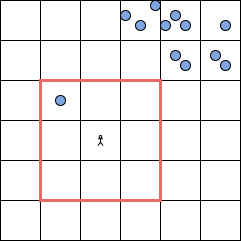
\includegraphics[scale=1]{decoupage_region.png}
    \caption{Exemple de cas où l'optimisation par découpage en régions est très utile.}
    \label{fig:decoupage_region}
\end{figure}

\paragraph{}
Dans la figure \ref{fig:decoupage_region} on observe que la plupart des entités sont loin de l'individu au centre, l'optimisation par régions permet de ne pas les prendre en compte et donc de ne faire des calculs
de collision avec que les objets dans la zone de perception de l'individu.
Nous avons implémenté ce découpage en permettant aux fourmis de récupérer les entités qui sont dans une certaine zone autour d'eux (en nombre de régions ou en distance réel dans le monde).
Cette optimisation nous a apporté un énorme gain en performances et a notamment rendu la présence d'un grand nombre de fourmis et de phéromone peu impactant sur les performances.

\subsubsection{Structures de données}
Un autre élément important dans l'optimisation de la simulation a été le choix des structures de données.

\section{Application}

\section{Tests}

\chapter{Résultats et perspectives}

\section{État des lieux}
\section{Apports}

\section{Évolutions possibles}


%--------------------------------------------------------------------------------
\chapter*{Conclusion}
\addcontentsline{toc}{chapter}{\numberline{}Conclusion}
\markboth{Conclusion}{}
 ultricies ut accumsan magna interdum. Nullam ut malesuada urna. Donec ut sem est. Curabitur ut neque elit. Sed aliquam sodales libero ut rutrum. Duis eu massa quam, rutrum posuere sapien. Suspendisse turpis nulla, eleifend ut faucibus consequat, laoreet varius tortor. Vestibulum accumsan sagittis hendrerit. Nunc tristique ligula quis ligula faucibus adipiscing. Aenean interdum, odio at volutpat interdum, justo nunc tristique elit, quis elementum nisi ante id arcu. Mauris commodo posuere cursus. Ut nec massa odio. Maecenas at eros arcu, quis rhoncus magna. Sed pellentesque dictum nulla nec pretium.

%--------------------------------------------------------------------------------
%exemple de bibliographie
\begin{thebibliography}{99}
\label{sec:biblio}
\bibitem{ref1}  détail bibliographique de la ref1
\bibitem{ref2}  détail bibliographique de la ref2
\bibitem{ref3}  détail bibliographique de la ref3
\bibitem{ref4}  détail bibliographique de la ref4
\bibitem{ref5}  détail bibliographique de la ref5
\end{thebibliography}


%--------------------------------------------------------------------------------
%si on donne des annexes :
\appendix
\addcontentsline{toc}{part}{\numberline{}Annexes}

%--------------------------------------------------------------------------------

\chapter{Liens utiles\label{sec:liens_utiles}}
Voici une petite liste d'url intéressantes au sujet de ce projet :

\begin{itemize}
\item {\url{https://github.com/PolyNoradrenalin/AntSimulator} Répertoire GitHub du projet}
\end{itemize}

%--------------------------------------------------------------------------------
%index : attention, le fichier dindex .ind doit avoir le même nom que le fichier .tex
%\printindex

%--------------------------------------------------------------------------------
%page du dos de couverture :

\resume{Integer lorem purus, rutrum quis lacinia in, egestas ut urna. Donec elementum mi id nisi blandit quis ultricies risus semper. Nulla congue tincidunt diam, id tincidunt mauris euismod nec. Nullam faucibus dapibus eros, at consequat odio rutrum quis. Curabitur nisl sem, suscipit in mattis eu, varius a mauris. Ut a augue ac augue fringilla egestas. Etiam non augue felis, in convallis nisi. Maecenas id urna ut justo tempor laoreet in eu ligula. Duis non erat vitae eros rhoncus rutrum sit amet at lorem. Ut tempor cursus ligula, eu bibendum ligula adipiscing eu. Fusce feugiat aliquam dolor, nec interdum nisl convallis vitae.}

\motcles{???, ????, ?????, ?????????, ??, ????}

\abstract{Integer lorem purus, rutrum quis lacinia in, egestas ut urna. Donec elementum mi id nisi blandit quis ultricies risus semper. Nulla congue tincidunt diam, id tincidunt mauris euismod nec. Nullam faucibus dapibus eros, at consequat odio rutrum quis. Curabitur nisl sem, suscipit in mattis eu, varius a mauris. Ut a augue ac augue fringilla egestas. Etiam non augue felis, in convallis nisi. Maecenas id urna ut justo tempor laoreet in eu ligula. Duis non erat vitae eros rhoncus rutrum sit amet at lorem. Ut tempor cursus ligula, eu bibendum ligula adipiscing eu. Fusce feugiat aliquam dolor, nec interdum nisl convallis vitae.}

\keywords{???, ????, ?????, ?????????, ??, ????}


\makedernierepage


\end{document}
%%FIN du fichier